%%%%%%%%%%%%%%%%%%%%%%%%%%%%%%%%%%%%%%%%%%%%%%%%%%%%%%%%%%%%%%%%%%%%
% Grundlagen
%%%%%%%%%%%%%%%%%%%%%%%%%%%%%%%%%%%%%%%%%%%%%%%%%%%%%%%%%%%%%%%%%%%%

\chapter{Material and Methods}
\label{matmet}

- Material: Was ich für ein Datensatz zum Testen benutzt habe und wo der herkommt
\label{lab:matmet:dataset}

\section{Implementation of the percolator algorithm}
- Wichtige Punkte wären:\\
- Verwendete Scipy-Methoden\\
- Abbruch wenn es nicht besser wird und dass ich die AUC als Metrik nutze\\
- \label{lab:matmet:normalization} feature normalization\\
- Wichtige Hilfsfunktionen (pseudoROC zB)\\
- Heißt jetzt Pycolator

\section{Adapting Percolator to Cross-link Identification}
To be able to monitor the difference any experiment makes, especially with respect to the cross-linked or non-cross-linked PSMs, following features were implemented:\\
First, in addition to the q-value, which is calculated as described in~\ref{background}, the calculation of a class-specific q-value was implemented. This is done by splitting the dataset according to the class affiliation and calculating the q-value separately for both splits.\\
Secondly, a ROC curve using the \emph{pseudoROC} function is calculated after every iteration of Percolator, for the whole dataset, only for cross-linked and only for non-cross-linked PSMs. Accordingly, the respective class-specific q-value is used. Thus, three plots containing the corresponding class(es) and every iteration are shown. This allows for fast visual detection of the impact a specific change to the algorithm has on certain classes, iterations or general sensitivity.
\subsection{Different Ranks}
As experience shows, cross-linked peptides can be harder to detect than linear peptides. This means, the possibly correct cross-linked peptide will frequently not get the highest score of all the peptides. It thus can be beneficial to not only consider the highest scoring peptide, but also the highest scoring cross-linked peptide or also some lower-scoring peptides and assign them ranks. Then, as experiments showed, Percolator can correct the scores of some lower-ranking PSMs, possibly detecting more cross-linked PSMs. Meanwhile, it is known to the experimenter, that only one of the peptides can be the correct match to a spectrum, and thus any PSM with a lower rank than 1 should be excluded at the end.\\
To tackle both constraints, Pycolator first trains the SVM with every PSM available and re-calculates the ranks based upon the newly assigned score, possibly correcting the ranks of some PSMs. When the used metric, normally the area under the curve of the pseudo ROC, does not improve beyond a certain threshold per iteration, every PSM with rank $2+$ is dropped. The threshold is controlled by the parameter \texttt{cutOffImprove} with a default of $0.01$ corresponding to a $1\%$ increase of the used metric per iteration. Since also some of the best scoring PSMs will be dropped, the algorithm then runs some more iterations in order to properly integrate and score the new PSMs considered confident.
\subsection{Characteristics of Cross-linked PSMs}
Apart from being hard to detect, cross-linked peptides also have other characteristics, some of which pose problems to the computational detection of correct PSMs. As discussed in~\ref{lab:matmet:splitting}, the features of cross-linked and linear peptides are so dissimilar, splitting the dataset and training a linear SVM separately on cross-links and non-cross-links yields significantly better results than training one linear SVM. To reduce the impact of this heterogeneity, the following experiments were conducted:
\subsubsection{Proportions of Different Classes}
\label{lab:matmet:proportions}
As discussed in~\ref{lab:background:percolator}, Percolator employs a nested cross-validation approach, splitting the dataset, training on all parts than one and testing/scoring on the remaining part. If the splitting was uneven by chance, the SVM would be trained badly and the scoring inaccurate. Having different classes with significant differences in the dataset, like in our case cross-linked and linear PSMs or targets and decoys, increases this problem. For example, if there was a testing split with many cross-linked PSMs, the SVM had to be trained on the remaining data with few cross-linked PSMs, resulting in probably poor scoring of the many cross-linked PSMs in the test set. In the average case, this should not be a problem, but it can produce on occasion worse or better results, following from overfitting.\\
To solve this problem, a mechanism of maintaining the proportion of the classes in the whole dataset for every inner and outer split was implemented. It can be toggled for targets and decoys or cross-linked and non-cross-linked PSMs as well as for inner and outer split independently. The impact has been measured by running the algorithm $10$ times, plotting and recording the results of the best, worst and median run w.r.t. to the AUC of the pseudo ROC curve. Because this took approximately 90 minutes, the test was performed in a Google Colaboratory notebook\footnote{The Google Colaboratory notebook used:\\ https://colab.research.google.com/drive/1VqZAmdta57YhgobA0WkQMqe\_U9YIUnDl?usp=sharing}.
%\begin{figure}
%	\label{fig:fluctuation_of_percolator}
%	\centering
%	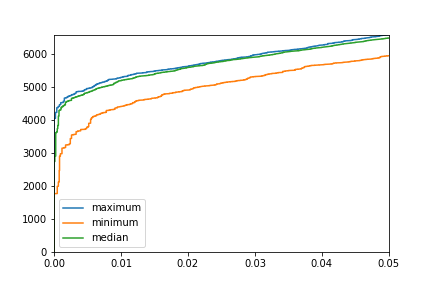
\includegraphics[width = 0.7\textwidth]{figures/percolator_MaxMinMedian_ClassesOption=.png}
%	\caption[Fluctuation of an earlier version of Percolator]{Pseudo ROC curve of an earlier version of the Percolator algorithm. It was run $10$ times and the best, worst and median run were plotted. Although the best run is close to the median one, the worst run is off by almost $1000$ PSMs. }
%\end{figure}
\subsubsection{Imputation}
\label{lab:matmet:imputation}
Cross-linked PSMs naturally have features linear PSMs do not have, which can however be used for training the SVM. An example would be the nucleotide it was linked to. BESSERES BEISPIEL S. MAIL. In the dataset given~\ref{lab:matmet:dataset}, $16$ of $61$ features were only given for cross-linked PSMs. Optimally, these should not influence the score a non-cross-linked PSM gets. However, $0$ was filled in for the missing values and because that is a valid value for the linear SVM, it biases the decision made. For example, if a high value in a feature leads the SVM to a decision against the PSM, $0$ as the lowest value possible after feature normalization~\ref{lab:matmet:normalization}, will tell the SVM to give the PSM a higher score, based on an actually missing feature.
%\footnote{https://scikit-learn.org/stable/modules/impute.html}
However, the scikit-learn package provides solutions for this problem\footnote{https://scikit-learn.org/stable/modules/impute.html}, and one of these, the \texttt{IterativeImputer}, was tested. % with Pycolator and the dataset~\ref{lab:matmet:dataset}
\subsubsection{Splitting the Dataset}
\label{lab:matmet:splitting}
- Trennung von Datensatz nach XL/nXL oder sogar cross-linking target falls Datensatz groß genug\\
\subsection{Small datasets}
- Ratio Testing (nicht-random aus ganzem Datensatz und random aus Top 10\%. Liefert Erkenntnisse über die mögliche Größe des Datensatzes und eventuell die Sinnhaftigkeit, wann man die Datensätze einfach trennen kann $\rightarrow$ Für den Leser relevant)\\
- Einbau von Identifikationen bei 1\% FDR als Metrik (Sinnhaftigkeit kann man ja diskutieren)\\\\			
(- Performance auf anderem Datensatz\\
- Vergleich mit Entrapment FDR)

%{
%\renewcommand{\baselinestretch}{0.9} 
%\normalsize
%\begin{table}[htb]
%\begin{tabular}{|c|}
%\end{tabular}
%  \caption[Tabellenverzeichnis]{}
%  \label{tab:1}
%\end{table}
%}